

\tikzset{every picture/.style={line width=0.75pt}} %set default line width to 0.75pt        

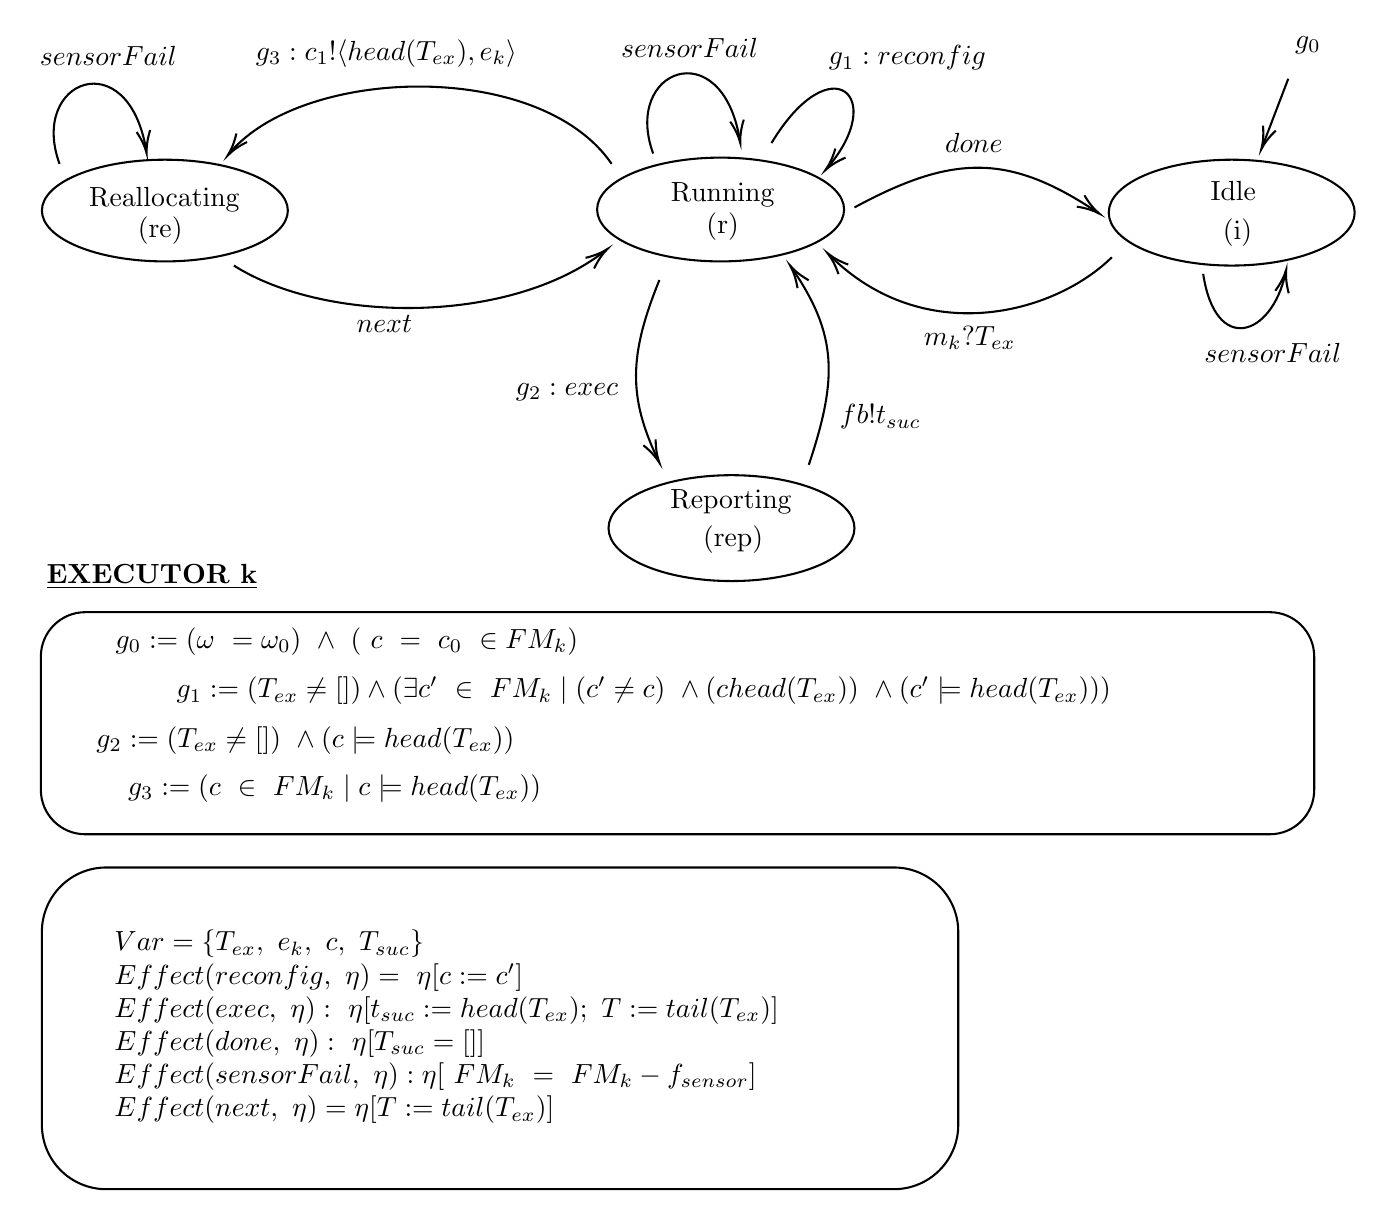
\begin{tikzpicture}[x=0.75pt,y=0.75pt,yscale=-1,xscale=1]
%uncomment if require: \path (0,582); %set diagram left start at 0, and has height of 582

%Curve Lines [id:da9480858267519683] 
\draw    (385.5,222) .. controls (399.29,180.63) and (399.5,159.63) .. (377.52,127.48) ;
\draw [shift={(376.5,126)}, rotate = 415.12] [color={rgb, 255:red, 0; green, 0; blue, 0 }  ][line width=0.75]    (10.93,-3.29) .. controls (6.95,-1.4) and (3.31,-0.3) .. (0,0) .. controls (3.31,0.3) and (6.95,1.4) .. (10.93,3.29)   ;
%Shape: Ellipse [id:dp6594609066072359] 
\draw   (283.5,99) .. controls (283.5,85.19) and (310.14,74) .. (343,74) .. controls (375.86,74) and (402.5,85.19) .. (402.5,99) .. controls (402.5,112.81) and (375.86,124) .. (343,124) .. controls (310.14,124) and (283.5,112.81) .. (283.5,99) -- cycle ;
%Shape: Ellipse [id:dp873836537729809] 
\draw   (530,100.5) .. controls (530,86.42) and (556.53,75) .. (589.25,75) .. controls (621.97,75) and (648.5,86.42) .. (648.5,100.5) .. controls (648.5,114.58) and (621.97,126) .. (589.25,126) .. controls (556.53,126) and (530,114.58) .. (530,100.5) -- cycle ;
%Curve Lines [id:da21020703050779688] 
\draw    (367.5,67) .. controls (396.21,19.48) and (423.94,44.49) .. (394.41,78.95) ;
\draw [shift={(393.5,80)}, rotate = 311.53] [color={rgb, 255:red, 0; green, 0; blue, 0 }  ][line width=0.75]    (10.93,-3.29) .. controls (6.95,-1.4) and (3.31,-0.3) .. (0,0) .. controls (3.31,0.3) and (6.95,1.4) .. (10.93,3.29)   ;
%Straight Lines [id:da37650774099478246] 
\draw    (616.5,36) -- (604.21,68.13) ;
\draw [shift={(603.5,70)}, rotate = 290.92] [color={rgb, 255:red, 0; green, 0; blue, 0 }  ][line width=0.75]    (10.93,-3.29) .. controls (6.95,-1.4) and (3.31,-0.3) .. (0,0) .. controls (3.31,0.3) and (6.95,1.4) .. (10.93,3.29)   ;
%Shape: Ellipse [id:dp02234558999259495] 
\draw   (16,99.5) .. controls (16,85.97) and (42.53,75) .. (75.25,75) .. controls (107.97,75) and (134.5,85.97) .. (134.5,99.5) .. controls (134.5,113.03) and (107.97,124) .. (75.25,124) .. controls (42.53,124) and (16,113.03) .. (16,99.5) -- cycle ;
%Curve Lines [id:da2517277021570281] 
\draw    (290.5,77) .. controls (255.85,26.51) and (141.81,29.93) .. (106.54,71.72) ;
\draw [shift={(105.5,73)}, rotate = 308.33000000000004] [color={rgb, 255:red, 0; green, 0; blue, 0 }  ][line width=0.75]    (10.93,-3.29) .. controls (6.95,-1.4) and (3.31,-0.3) .. (0,0) .. controls (3.31,0.3) and (6.95,1.4) .. (10.93,3.29)   ;
%Curve Lines [id:da851947022127026] 
\draw    (108.5,126) .. controls (152.06,153.72) and (240.7,154.98) .. (287.11,119.1) ;
\draw [shift={(288.5,118)}, rotate = 501.19] [color={rgb, 255:red, 0; green, 0; blue, 0 }  ][line width=0.75]    (10.93,-3.29) .. controls (6.95,-1.4) and (3.31,-0.3) .. (0,0) .. controls (3.31,0.3) and (6.95,1.4) .. (10.93,3.29)   ;
%Curve Lines [id:da05773774536505705] 
\draw    (531.5,122) .. controls (503.29,149.72) and (440.77,165.68) .. (395.86,121.36) ;
\draw [shift={(394.5,120)}, rotate = 405.63] [color={rgb, 255:red, 0; green, 0; blue, 0 }  ][line width=0.75]    (10.93,-3.29) .. controls (6.95,-1.4) and (3.31,-0.3) .. (0,0) .. controls (3.31,0.3) and (6.95,1.4) .. (10.93,3.29)   ;
%Rounded Rect [id:dp5913972444482631] 
\draw   (15.5,314.4) .. controls (15.5,302.58) and (25.08,293) .. (36.9,293) -- (607.6,293) .. controls (619.42,293) and (629,302.58) .. (629,314.4) -- (629,378.6) .. controls (629,390.42) and (619.42,400) .. (607.6,400) -- (36.9,400) .. controls (25.08,400) and (15.5,390.42) .. (15.5,378.6) -- cycle ;
%Rounded Rect [id:dp9206164489184118] 
\draw   (16,447) .. controls (16,429.88) and (29.88,416) .. (47,416) -- (426.5,416) .. controls (443.62,416) and (457.5,429.88) .. (457.5,447) -- (457.5,540) .. controls (457.5,557.12) and (443.62,571) .. (426.5,571) -- (47,571) .. controls (29.88,571) and (16,557.12) .. (16,540) -- cycle ;
%Curve Lines [id:da46585089178877326] 
\draw    (24.5,77) .. controls (9.65,36.41) and (57.53,18.36) .. (66.25,70.4) ;
\draw [shift={(66.5,72)}, rotate = 261.57] [color={rgb, 255:red, 0; green, 0; blue, 0 }  ][line width=0.75]    (10.93,-3.29) .. controls (6.95,-1.4) and (3.31,-0.3) .. (0,0) .. controls (3.31,0.3) and (6.95,1.4) .. (10.93,3.29)   ;
%Curve Lines [id:da24525569786800605] 
\draw    (575.5,130) .. controls (581.38,169.2) and (608.39,160.38) .. (615.11,129.89) ;
\draw [shift={(615.5,128)}, rotate = 460.62] [color={rgb, 255:red, 0; green, 0; blue, 0 }  ][line width=0.75]    (10.93,-3.29) .. controls (6.95,-1.4) and (3.31,-0.3) .. (0,0) .. controls (3.31,0.3) and (6.95,1.4) .. (10.93,3.29)   ;
%Curve Lines [id:da5617910694928671] 
\draw    (310.5,72) .. controls (295.65,31.41) and (343.53,13.36) .. (352.25,65.4) ;
\draw [shift={(352.5,67)}, rotate = 261.57] [color={rgb, 255:red, 0; green, 0; blue, 0 }  ][line width=0.75]    (10.93,-3.29) .. controls (6.95,-1.4) and (3.31,-0.3) .. (0,0) .. controls (3.31,0.3) and (6.95,1.4) .. (10.93,3.29)   ;
%Shape: Ellipse [id:dp893416141673501] 
\draw   (289,252.5) .. controls (289,238.42) and (315.53,227) .. (348.25,227) .. controls (380.97,227) and (407.5,238.42) .. (407.5,252.5) .. controls (407.5,266.58) and (380.97,278) .. (348.25,278) .. controls (315.53,278) and (289,266.58) .. (289,252.5) -- cycle ;
%Curve Lines [id:da2982425830385871] 
\draw    (313.5,133) .. controls (298.72,169.45) and (298.5,189.4) .. (312.84,219.61) ;
\draw [shift={(313.5,221)}, rotate = 244.18] [color={rgb, 255:red, 0; green, 0; blue, 0 }  ][line width=0.75]    (10.93,-3.29) .. controls (6.95,-1.4) and (3.31,-0.3) .. (0,0) .. controls (3.31,0.3) and (6.95,1.4) .. (10.93,3.29)   ;
%Curve Lines [id:da08998093824564413] 
\draw    (407.5,98) .. controls (455.02,72.26) and (481.96,72) .. (524.21,100.14) ;
\draw [shift={(525.5,101)}, rotate = 214] [color={rgb, 255:red, 0; green, 0; blue, 0 }  ][line width=0.75]    (10.93,-3.29) .. controls (6.95,-1.4) and (3.31,-0.3) .. (0,0) .. controls (3.31,0.3) and (6.95,1.4) .. (10.93,3.29)   ;

% Text Node
\draw (344,92) node   [align=left] {Running};
% Text Node
\draw (590,90) node   [align=left] {Idle};
% Text Node
\draw (420,199) node    {$fb!t_{suc}$};
% Text Node
\draw (182,24) node    {$g_{3} :c_{1} !\langle head( T_{ex}) ,e_{k} \rangle $};
% Text Node
\draw (463,161) node    {$m_{k} ?T_{ex}$};
% Text Node
\draw (75,94) node   [align=left] {Reallocating};
% Text Node
\draw (181,154) node    {$next$};
% Text Node
\draw (306,331) node    {$g_{1} :=( T_{ex} \neq []) \land ( \exists c'\ \in \ \llbracket FM_{k} \rrbracket \mid ( c'\neq c) \ \land ( c\nvDash head( T_{ex})) \ \land ( c'\models head( T_{ex})))$};
% Text Node
\draw (433,26) node    {$g_{1} :reconfig$};
% Text Node
\draw (269,187) node    {$g_{2} :exec$};
% Text Node
\draw (143,355) node    {$g_{2} :=( T_{ex} \neq []) \ \land ( c\models head( T_{ex}))$};
% Text Node
\draw (152,461) node    {$ \begin{array}{l}
\end{array}$};
% Text Node
\draw (211,493) node    {$ \begin{array}{l}
Var=\{T_{ex} ,\ e_{k} ,\ c,\ T_{suc}\}\\
Effect( reconfig,\ \eta ) =\ \eta [ c:=c']\\
Effect( exec,\ \eta ) :\ \eta [ t_{suc} :=head( T_{ex}) ;\ T:=tail( T_{ex})]\\
Effect( done,\ \eta ) :\ \eta [ T_{suc} =[]]\\
Effect( sensorFail,\ \eta ) :\eta [ \ FM_{k} \ =\ FM_{k} -f_{sensor}]\\
Effect( next,\ \eta ) =\eta [ T:=tail( T_{ex})]
\end{array}$};
% Text Node
\draw (73,109) node   [align=left] {(re)};
% Text Node
\draw (344,107) node   [align=left] {(r)};
% Text Node
\draw (592,110) node   [align=left] {(i)};
% Text Node
\draw (626,20) node    {$g_{0}$};
% Text Node
\draw (157,378) node    {$g_{3} :=( \nexists c\ \in \ \llbracket FM_{k} \rrbracket \mid c\models head( T_{ex}))$};
% Text Node
\draw (163,307) node    {$g_{0} :=( \omega \ =\omega _{0}) \ \land \ ( \ c\ =\ c_{0} \ \in \llbracket FM_{k} \rrbracket )$};
% Text Node
\draw (48,25) node    {$sensorFail$};
% Text Node
\draw (609,168) node    {$sensorFail$};
% Text Node
\draw (465,67) node    {$done$};
% Text Node
\draw (328,21) node    {$sensorFail$};
% Text Node
\draw (348,240) node   [align=left] {Reporting};
% Text Node
\draw (349,258) node   [align=left] {(rep)};
% Text Node
\draw (69,276) node   [align=left] {\textbf{\underline{EXECUTOR k}}};


\end{tikzpicture}